\section{Аналіз та вибір навігаційного забезпечення}

Відповідно до розробленої у НДР „”( \text{[TODO добавить номер НДР]}) методики 
побудови комплексної навігаційної системи, задача створення 
інерціально-супутникової системи навігації для визначення координат 
місцеположення рухомого об'єкта, передбачає: (Дальше идет методика. 
В ней надо убрать все, что касается нанотехнологий и МЕМС датчиков)

Обґрунтування, та вибір (або розробка) структури і варіанту комплексування 
інтегрованої інерціально-супутникової системи на основі аналізу класу і 
технічних характеристик ЛА, з урахуванням діапазонів кутів крену та тангажа, 
ударних навантажень, максимальних швидкостей та прискорень, орієнтуючись на 
тип точності основних навігаційних засобів (комплекс середньої точності, 
низької вартості та малих габаритів і маси), масогабаритні характеристики, 
споживану потужність та вартість обладнання. 

Формулювання основних характеристик комплексної системи у вигляді граничних 
погрішностей навігаційних визначень;

Для обраного варіанту інтегрованої інерціально-супутникової системи 
обирається з представленого на ринку модельного ряду авіаційних 
приемоіндикаторів супутникових систем потрібний за технічними 
характеристиками та розв'язуваними задачами тип приемоіндикатора, або 
формулюються технічні вимоги  на розробку такого приемоіндикатора. 

Для обраного варіанту інерціально-супутникової системи обирається схема 
інерціальної навігаційної системи;

На основі аналізу варіантів побудови датчиків первісної інформації БІНС 
і основних характеристик інерціальных датчиків, використовуючи методику 
попереднього оцінювання точностних характеристик ДПІ БІНС, обираються типи 
датчиків первісної інформації БІНС;

Ґрунтуючись на аналізі типових польотних завдань, що виконує даний клас ЛА 
або БПЛА, обираються варіанти систем координат, в яких повинні формулюватися 
кінематичні рівняння алгоритмів БІНС;

Для обраних варіантів систем координат розробляються кінематичні рівняння 
алгоритмів БІНС, в яких при завданні орієнтацію зв'язаної системи координат 
відносно опорної за рішенням проектанта можуть бути використані алгоритми 
із застосуванням направляючих косинусів, кутів Ейлера, компонентів векторів 
кінцевого повороту й орієнтації, параметрів Родріга-Гамільтона, параметрів 
Келі-Клєйна;

Після прийняття рішення про корекцію вертикального каналу інтегрованої 
інерціально-супутникової системи від вимірника барометричної висоти обирається 
тип баровисотоміра, або формулюються технічні вимоги на розробку такого 
вимірника, обирається тип датчика статичного тиску, розробляються алгоритми 
обчислення барометричної висоти за інформацією від датчика статичного тиску;

Випереджаючи розробку алгоритмів комплексної обробки навігаційної 
інформації, виконується розробка математичних моделей похибок датчиків, 
БІНС, СНС та вимірника барометричної висоти. Причому, якщо за моделі 
похибок датчиків БІНС, СНС та вимірника барометричної висоти можна 
застосовувати відомі математичні моделі, то математичну модель похибок 
БІНС потрібно формулювати базуючись на розроблених алгоритмах ідеальної 
роботи БІНС;

Після прийняття рішення про застосування в інтегрованої інерціально-супутникової 
системі оптимальної схеми комплексування виконується розробка алгоритмів 
комплексної обробки навігаційної інформації від БІНС, СНС та вимірника 
барометричної висоти на базі процедур оптимальної дискретної калманівської 
фільтрації залежно від обраного варіанту схем інтегрування: для слабкозвязаної 
або сильнозвязаної системи, з метою оцінювання похибок і введення поправок у 
вихідні дані БІНС.
% 
% З метою забезпечення стійкої роботи інтегрованої навігаційної системи з
% оптимальною схемою комплексування за запропонованою методикою викону­ється
% розробка алгоритмів введення зворотних звязків у БІНС за результатами 
% оцінювання її похибок та калібрування датчиків БІНС.
% 
% Для підтвердження працездатно­сті та ефективності запропонованих рішень 
% виконується імітаційне математичного моделювання інтегрова­ної інформаційної 
% системи в польоті з використанням аналітичного завдання еталонних параметрів 
% руху ЛА в функції часу.

\subsection{Аналіз та вибір структури та варіанту комплексуванн інегрованої
інерціально-супутникової системи}

В теперішній час розроблені схеми можливого комплексування СНС і ІНС у чотирьох 
основних варіантах:
\begin{enumerate}
\item роздільна схема;
\item слабко зв'язана схема;
\item жорстко зв'язана схема;
\item глибоко інтегрована схема.
\end{enumerate}

Тут і в подальшому під СНС мається на увазі інтегрована СНС ГЛОНАСС/GPS. 

Перший варіант -- це роздільна або розімкнута схема \ref{fig:isns_break}.  Це  найбільш 
простий варіант спільного використання ІНС і СНС. Тут обидві системи працюють незалежно 
одна від одної, але, оскільки похибки ІНС з часом зростають, то необхідно періодично
або безперервно проводити корекцію ІНС за даними СНС. Для демпфірування вертикального 
каналу ІНС може бути застосована інформація від системи повітряних сигналів (СПС).

\begin{figure}[here]
\centering
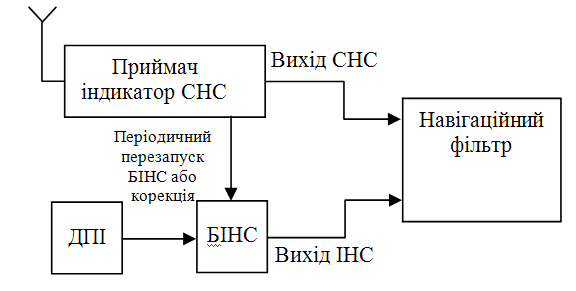
\includegraphics{sns_break}
\caption{Розімкнута схема}
\label{fig:isns_break}
\end{figure}

Періодична корекція може зводитися до періодичного перезапуску алгоритму ІНС із новими 
початковими умовами за координатами та швидкістю, дані про які надходять від приймача СНС. 
Безперервна корекція процедурно може бути оформлена як одночасна позиційна та 
швидкісна корекції ІНС за сигналами СНС. Така архітектура комплексування на  
етапі розв'язання навігаційної задачі (на етапі вторинної обробки інформації) 
забезпечує незалежність систем (крім моментів  перезапуску або корекції) й 
інформаційну надмірність сукупної структури. Вихідна інформація двох систем може 
піддаватися комплексній обробці з використанням калманівської фільтрації.

В цілому комплексна система має більш високу точність як за координатами та швидкістю, 
так і за кутовою орієнтацією. При цьому зберігається можливість одержувати позиційну, 
швидкісну та кутову інформацію (у тому числі про перевантаження та кутову швидкість), 
необхідну для цілей пілотування та навігації з високою частотою, притаманною ІНС.

Крім того, для створення  архітектури такої інтегрованої ІССН потрібні мінімальні зміни 
в апаратних засобах і програмному забезпеченні вже існуючого обладнання ЛА.

Наступною за глибиною зв'язку ІНС і СНС є слабко зв'язана система. Тут інерціальна 
система та приймач СНС як і раніше виробляють незалежні навігаційні вимірювання, 
однак з'являється з'єднувальний блок -- обчислювач ІНС СНС, у якому формується оцінка 
координат і швидкості польоту, виробляється корекція даних, отриманих від ІНС (рис. 
\ref{fig:isns_loosly}).

\begin{figure}[here]
\centering
\includegraphics[bb=0mm 0mm 208mm 296mm, width=109.7mm,height=93.3mm, viewport=3mm 4mm 205mm 292mm]{image4}
\caption{Розімкнута схема}
\label{fig:isns_loosly}
\end{figure}

В цій схемі функціональний розподіл підсистем може супроводжуватися їхнім фізичним 
поділом: приймач СНС, ІНС і навігаційний обчислювач конструктивно оформляються у 
вигляді закінчених роздільних блоків, між якими організовані відповідні інформаційні 
зв'язки, що не вимагають, як правило, високих швидкостей передачі даних. Зрозуміло, 
усі три перелічені компоненти системи можуть бути розміщені й у єдиному модулі, якщо 
це бажано за умовами функціонування комплексу.

У слабко зв'язаних системах ІНС повинна забезпечити досить тривале функціонування 
зі  збереженням прийнятної точності.  Таким  чином, передбачається можливість як 
роздільного функціонування ІНС і СНС протягом тривалого періоду, так і їх сумісного 
функціонування в інтегрованому режимі. 

У СНС  (див. рис. \ref{fig:isns_loosly}) сигнал, прийнятий антенним блоком, є сигналом несучої частоти,  
модульованим за амплітудою псевдовипадковим сигналом тривалістю  $dt \approx$ 1 мксек 
(або 300 м еквівалентної довжини коду). Вхідні сигнали демодулюються і подаються 
на корелятори.  Інформація з кореляторів передається в контури слідкування за фазою 
(КСФ) і затримкою (КСЗ). Контур слідкування за затримкою видає командні сигнали, 
які здійснюють  затримку або випередження сигналів на виході корелятора (див. [+, --] 
на рис. \ref{fig:isns_loosly}) доти, поки на виході корелятора не з'явиться сигнал максимальної величини, 
а різниця сигналів корелятора на попередньому і поточному кроках не буде дорівнювати 
нулю. Це означає „захоплення'' сигналу супутника, а величина отриманої при цьому 
затримки  вважається часом поширення сигналу від супутника до приймача і використовується 
для обчислення псевдодальності $\dot{R}_{i}$ до конкретного супутника. Синфазна та 
квадратурна складові сигналів несучої частоти ($IQ$ відповідно -- на рис. \ref{fig:isns_loosly}) 
подаються в контур слідкування за фазою несучої частоти (КСФ). Арктангенс 
пропорційний амплітуді квадратурного (\textit{Q}) сигналу до синфазного (\textit{I} ) 
є похибкою КСФ. Цей сигнал похибки подається у вигляді зворотного зв'язку в корелятор, 
здійснюючи фазове автопідстроювання його частоти. Різниця частот опорного і прийнятого 
сигналів пропорційна швидкості зміни псевдодальності  $\dot{R}_{i} $. При цьому
контур КСФ має астатизм 3-го порядку, що дозволяє відслідковувати 
сигнали з постійним прискоренням (другої похідної від псевдодальності). Якщо цей 
контур захоплює і стежить за фазою, він подає коригувальний сигнал $\Delta R$ у 
контур КСЗ, підвищуючи тим самим точність визначення псевдодальності \textit{R}. 

 Інформація 
про вимірювані псевдодальності \textit{R} і псевдошвидкості $\dot{R}_{i} $ використовується 
в алгоритмах розв'язання навігаційних задач для отримання координат і швидкості споживача, 
а також виправлень до еталона часу та частоти приймача СНС. При наявності надмірності 
з метою підвищення точності зчислення навігаційних параметрів здійснюється їхнє спільне 
оцінювання, зокрема з використанням оптимальної калманівської  фільтрації. 

Робота супутникової системи коригується від ІНС на етапі ``холодного'' і ``гарячого'' 
стартів.\textbf{ }Тут приймач СНС використовує інформацію від ІНС тільки з метою 
більш надійного та швидкого відновлення захоплення сигналу у випадку його втрати. 
На схемі це показано зв'язком вихідного блоку ІНС і корелятора. Передана по цьому 
каналу інформація про обчислені координати та швидкість ЛА у випадку втрати слідкування 
дозволяє розрахувати оцінки передбачуваної затримки сигналу $\tau$ та доплерівського 
зсуву частоти несучої $f_{\text{доп}}$, що суттєво знижує час пошуку та захоплення сигналу. 
В результаті значно знижується час 
відновлення роботи приймача після втрати сигналу, тобто тут в деякому смислі реалізоване 
об'єднання ІНС і СНС не тільки на рівні вторинної обробки інформації, а й на рівні 
первинної обробки радіосигналів. 

У блоці ІНС на рис. \ref{fig:isns_loosly} показана структура безплатформної інерціальної системи. 
Блок датчиків видає вектори кутових  швидкостей $\omega$ та лінійних прискорень \textit{а}. 
У блоці „кінематика обертового руху'' виконується інтегрування кінематичних рівнянь 
кутового руху та формується матриця напрямних косинусів \textit{В} за інформацією 
датчиків кутових швидкостей. Матриця напрямних косинусів \textit{В} разом із даними 
акселерометрів використовується в блоці інтегрування кінематичних рівнянь поступального 
руху -- блок ``кінематика поступального руху''. На виході цього блоку формуються 
координати та швидкості ЛА у вибраній навігаційній системі.

У середній частині рис. \ref{fig:isns_loosly} зображено з'єднувальний блок -- обчислювач ІНС СНС, 
що копіює алгоритм безплатформної ІНС, здійснює в блоці „компенсатор похибок датчиків'' 
компенсацію похибок датчиків відповідно до моделей цих похибок та реалізує безпосередньо 
комплексування ІНС і СНС. Оцінка параметрів, що характеризують фазові координати 
руху ЛА, реалізується в польоті за результатами, наприклад, розширеної калманівської 
фільтрації сигналів ІНС і СНС у блоці ФК. За результатами оцінювання здійснюється 
позиційна та швидкісна корекція копії алгоритмів безплатформної ІНС. Корекція самої 
ІНС у слабко-зв'язаних системах не передбачається. Але в ІНС передбачається можливість 
компенсації інструментальних похибок вимірювальних елементів за апріорними даними 
(наприклад, за паспортними даними  системи) або за значеннями оцінок цих похибок, 
що отримані в обчислювачі ІНС СНС. В результаті в основний алгоритм ІНС передаються 
скориговані показання датчиків кутової швидкості і акселерометрів.

Як видно, у слабко зв'язаній системі навігаційні параметри, так само як і в роздільній 
схемі, виробляються незалежно як у ІНС так і в СНС, причому, як уже відзначалося, 
до складу приймача включена схема оцінювання (як правило, фільтр Калмана). Така схема 
зветься „каскадною'' через два послідовно включених фільтри Калмана. Достоїнством 
такої схеми є висока надійність інтегрованої системи, а недоліком -- взаємна кореляція 
похибок оцінок першого фільтра (фільтра супутникового приймача) і їх відмінність 
від білих шумів. Надходячи з виходу СНС на вхід другого фільтра Калмана, і стаючи 
для нього шумами вимірювань, вони порушують умови оптимальної роботи цього фільтра. 
Крім цього, у такій схемі необхідно здійснювати заходи синхронізації вимірювань ІНС 
і приймача СНС.

Підвищений рівень автономності ІНС (передбачається, що підсистема ІНС може працювати 
автономно протягом 1-ї години) вимагає значної точності інерціальних датчиків (датчиків 
кутових швидкостей і акселерометрів) і застосування досить складних алгоритмів інерціальної 
навігації. Тому такі системи досить дорогі та складні. Такі системи доцільно застосовувати 
в ПНК високої та середньої точності, але, наприклад для БПЛА, вони занадто дорогі.

У літературі можна знайти ділення слабко зв'язаних схем на три типи: стандартну, агресивну 
і так звану \textit{MAGR}-схему (\textit{Military Airborne GPS Receiver}). Відмінність 
„агресивної'' схеми від стандартної полягає в тому, що в ній використовується інформація 
БІНС про прискорення для екстраполяції навігаційних вимірювань приймача СНС в період 
між супутниковими вимірюваннями. \textit{MAGR} - схема фірми \textit{Rockwell} використовує 
інерціальні вимірювання в контурі слідкування за кодом СНС-приймача при провалі „захоплення'' 
у контурі слідкування за несучою частотою. У цьому випадку можна говорити про повноцінне 
комплексування як на рівні вторинної обробки інформації, так й на рівні первинної 
обробки інформації.

Третій варіант інтеграції систем -- жорстко зв'язана схема (рис. \ref{fig:isns_tide}).
У жорстко зв'язаних системах ступінь автономності ІНС значно менший, ніж у слабко зв'язаних 
системах: допускається автономна робота протягом від декількох секунд до декількох 
десятків секунд. Практично в цих системах ІНС найчастіше є придатком для СНС. Основна 
навігаційна інформація виробляється в СНС, у той час як ІНС інтерполює значення навігаційних 
параметрів у період між двома сусідніми тактами надходження інформації від СНС, а 
також забезпечує навігаційною інформацією системи керування польотом при короткочасній 
втраті сигналів від супутників. 

ІНС у жорстко зв'язаних системах забезпечує „сирі вимірювання''. Блок датчиків видає 
вектори кутових  і лінійних координат.  

Компенсація похибок датчиків відповідно до моделей цих похибок виконується в блоці 
компенсатора похибок від розширеного фільтра Калмана. Інтегрування кінематичних рівнянь 
обертового руху та поступального руху виконується з урахуванням скоригованих координат. 
Тобто в у жорстко зв'язаних системах виконується одночасно процедури оцінювання (фільтрації) 
і коригування ІНС.
\begin{figure}[here]
\centering
\includegraphics[bb=0mm 0mm 208mm 296mm, width=115.1mm, height=72.0mm, viewport=3mm 
4mm 205mm 292mm]{image1.eps}
\caption{Жорстко зв'язана схема інтегрування}
\label{fig:isns_tide}
\end{figure}

Приймач СНС функціонує аналогічно описаному вище варіанту 
слабко зв'язаної схеми. Відмінністю даної структури від попередніх є відсутність 
у складі приймача фільтра Калмана. У жорстко зв'язаній схемі ІНС і приймач лише забезпечують 
склад вимірювань для загального обчислювального блоку, в якому реалізований єдиний 
фільтр Калмана. Вимірювання для фільтра в жорстко зв'язаних системах будуються за 
різницею псевдодальностей або/і швидкостей зміни псевдодальностей, визначених, з 
одного боку, в ІНС за обчисленими координатами ЛА й ефемеридами супутника, і вимірюваними 
приймачем-індикатором СНС, з іншого. При цьому за навігаційну систему координат ІНС 
доцільно вибирати ту систему координат, в якій працює СНС.  

Фільтр Калмана, на відміну від попереднього випадку, повинен бути дуже швидкодіючим. 
Це пов'язано з тим, що зв'язок блока фільтра Калмана з контурами приймача СНС значно 
більш жорсткий, ніж у попередньому випадку, оскільки відмінною рисою жорстко зв'язаної 
схеми є використання контурами слідкування за затримкою і фазою інформації про розрахункові 
псевдодальності і псевдошвидкості (або про їхні збільшення), які надходить саме від 
фільтра Калмана. Використання цієї інформації дозволяє істотно поліпшити стійкість 
слідкування і знизити час відновлення роботи приймача у випадку втрати сигналів супутників. 
Необхідно, щоб ці дані надходили з високою швидкістю так, щоб період часу між вимірюваннями 
в підсистемі СНС був розбитий на велику кількість підінтервалів  з метою корекції 
контурів слідкування. Це потрібно для того, щоб постачати контуру слідкування інформацію 
навіть тоді, коли вхідний сигнал приймача відсутній або подавлений завадами, тобто 
тут реалізоване повномасштабне комплексування ІНС/СНС і на рівні первинної обробки 
інформації.

Жорстко зв'язані системи мають більшу точність при тих самих інерціальних датчиках 
у порівнянні зі слабко зв'язаними системами. У цих системах за рахунок додаткових 
сигналів корекції від  ІНС смуга пропускання контурів слідкування СНС може бути значно 
зменшена. При цьому зростає завадостійкість цих систем і зменшується ймовірність 
втрати сигналів, що відслідковуються. До того ж застосування фільтра Калмана, що 
відновлює повний вектор стану, включаючи  псевдодальність \textit{R} і швидкість 
її зміни $\dot{R}$, навіть при неповних вимірюваннях, дозволяє СНС працювати навіть 
при кількості видимих супутників менше 4-х. Якщо кількість цих супутників більше 
4-х, то фільтр Калмана здійснює комплексування інформації, що надходить від видимих 
супутників. Однак, наявність лише одного фільтра Калмана призводить до втрати надмірності 
системи, тому що стає доступним лише одне спільне рішення. 

Як і у слабко зв'язаних системах тут передбачено коригування СНС від коректованої 
ІНС на етапах „холодного'' та „гарячого'' стартів, а відновлені значення псевдодальності 
$\Delta$\textit{R}ф і швидкості її зміни $\Delta \dot{R}_{{\rm D}} $, надходячи в контури 
слідкування за затримкою КСЗ  та за фазою КСФ сигналу СНС, забезпечують процедуру 
інтерполяції.

Таким чином, основні відмінності жорстко зв'язаної схеми від слабко зв'язаної полягають 
у наступному:

\begin{enumerate}
\item використання вихідної інформації ІНС про прискорення в контурі слідкування 
за кодом і доплерівським зсувом несучої частоти, що дозволяє звузити смугу пропускання 
контурів слідкування і підвищити швидкодію та точність настроювання;
\item використання вимірювань псевдодальностей та псевдошвидкостей (а не координат 
і швидкостей) для оцінювання похибок ІНС.
\end{enumerate}

Як вже було зазначено, жорстко зв'язані системи забезпечують більш високу точність 
розв'язання навігаційної задачі в порівнянні зі слабко зв'язаними системами. До інших 
переваг такої схеми можна віднести:

\begin{enumerate}
\item відсутність проблем взаємної кореляції шумів вимірювань та їхніх відмінностей 
від білих шумів;
\item відсутність проблеми синхронізації вимірювань ІНС і СНС, оскільки використовується 
один формувач тактових частот;
\item можливість виявлення та відбраковування схиблених вимірювань псевдодальностей 
за їхніми передбачуваними значеннями, сформованими з використанням даних від ІНС.
\end{enumerate}

До недоліків жорстко зв'язаних систем можна віднести:

\begin{enumerate}
\item необхідність розробки спеціальної апаратури споживача (приймача-індикатора СНС);
\item використання складних співвідношень для вимірювань;
\item зниження надійності, оскільки відмова ІНС призводить до відмови системи в цілому;
\item відсутність надмірності, що ускладнює рішення задач діагностики та контролю.
\end{enumerate}

Два 
останні недоліки можна усунути, використовуючи фільтр Калмана в приймачі СНС і перераховуючи 
навігаційну інформацію скоригованої ІНС у навігаційну систему координат споживача.   
Таке рішення створює деякий проміжний варіант між слабко і жорстко зв'язаними схемами -- варіант 
інерціально-супутникової системи середньої інтеграції (рис.\ref{fig:isns_lootide}) .

\begin{figure}[here]
\centering
\includegraphics[bb=0mm 0mm 208mm 296mm, width=102.5mm, height=74.7mm, viewport=3mm 
4mm 205mm 292mm]{image2.eps}
\caption{Система середнього типу інтеграції}
\label{fig:isns_lootide}
\end{figure}

Система, що зображена на рис. \ref{fig:isns_lootide}, надає два навігаційних 
рішення: одне на виході блоку СНС, інше -- на виході ІНС. Блоки, що зображені на 
схемі рис. \ref{fig:isns_lootide}, мають той же зміст, що і на попередніх схемах. ІНС може забезпечувати 
розв'язання навігаційної задачі навіть при  відсутності сигналів від СНС. Крім того, 
передбачений режим підтримки роботи СНС від ІНС за рахунок поліпшення стійкості слідкування. 
Блок КЗФ -- блок слідкування за фазою  несучої частоти, зазвичай, більш уразливий 
для природних або штучних завад. Тому, якщо цей блок слідкування втратив „захоплення'' 
фази і не виконує функцію підтримки слідкування КЗС, тобто працює тільки блок КСЗ - 
блок слідкування за затримкою, то ІНС заміняє відсутній сигнал $\Delta$\textit{R} на 
сигнал $\dot{R}_{{\rm !}} $, підтримуючи, таким чином, роботу супутникової системи 
без збоїв.

ІНС у цьому випадку, так само як і у всіх інших, використовується також і для екстраполяції 
сигналів положення \textit{R} і швидкості $\dot{R}$між двома вимірюваннями СНС.

Оскільки у фільтрі Калмана відновлюється цілком весь вектор стану ЛА, то  змінні 
кутової орієнтації використовуються для корекції алгоритмів інтегрування кінематичних 
рівнянь кутового руху, тобто здійснюється корекція за швидкістю. 

Крім розглянутих варіантів структур комплексної системи, існують ще й інші варіанти, 
що побудовані як за принципом слабкої, так і жорсткої інтеграції. Але при цьому слід 
мати на увазі, що ці варіанти вимагають значно більш складного і дорогого математичного 
забезпечення в порівнянні з уже розглянутими варіантами структур.  

Так звані глибоко інтегровані системи є ще більш складними і менш гнучкими з огляду 
організації їхньої структури, мають жорстку організацію зв'язків і єдиний вихід (рис. 
10.5). 

Обчислювач ІНС/СНС реалізує алгоритми безплатформної ІНС й алгоритми оптимальної 
оцінки параметрів. Всі оцінки виробляються в інтегральному фільтрі Калмана, а приймач 
СНС ГЛОНАСС/GРS ще більш спрощується. У цій схемі він складається тільки з високочастотного 
каналу прийому і первинної обробки інформації, що включає високочастотний прийомний 
тракт, генератор коду, корелятори і схему „захоплення''. Виходи кореляторів є входами 
для інтегрального фільтра Калмана, де обчислюються не тільки похибки ІНС, але й оцінки 
псевдодальностей і псевдошвидкостей, які передаються в приймач для поліпшення характеристик 
„захоплення'' сигналу. Таким чином, традиційні контури слідкування за кодом і доплерівською 
частотою включаються в загальний інтегральний фільтр комплексної системи. У такій 
схемі фільтр повинен мати двадцятий-сороковий порядок, і для його реалізації потрібна 
БЦОМ із високою швидкодією.

Усі перераховані схеми комплексування СНС і ІНС (крім першої), одержують на виході 
фільтра Калмана оцінки інструментальних похибок ІНС (похибки зсуву нулів гіроскопів 
і акселерометрів, похибки масштабних коефіцієнтів і т. ін.), які використовуються 
для корекції інерціальних датчиків. Тому при перервах надходження даних із приймача 
отримані раніше оцінки похибок ІНС і її вимірювальних елементів дозволяють поліпшити 
точнісні характеристики ІНС в автономному режимі.

В табл. \ref{tab:compare} підсумовані основні особливості перелічених схем комплексних систем.

\begin{table}[here]
\centering
\caption{Особливості схем комплексування}
\label{tab:compare}
\begin{tabular}{|p{30mm}|p{110mm}|} \hline 
Тип системи & Основні особливості \\ \hline 
Роздільна & Надмірність, обмеженість похибок оцінок місця розташування і швидкості, 
наявність інформації про орієнтацію і кутову швидкість, висока швидкість видачі інформації, 
мінімальні зміни в бортовій апаратурі  \\ \hline 

Слабко\newline зв'язана & Усі перераховані особливості роздільних систем, плюс більш 
швидке відновлення слідкування за кодом і фазою сигналів СНС, виставлення та калібрування 
БІНС у польоті, як наслідок -- підвищена точність під час відсутності сигналу СНС  \\ \hline 

Жорстко зв'язана & Подальше поліпшення точності і калібрування, підвищена стійкість слідкування 
за сигналами СНС при маневрах ЛА, підвищена завадостійкість  \\ \hline
 
Глибоко інтегрована & Достоїнства: єдиний фільтр усуває проблему ``каскадного'' включення 
фільтрів, компактність, знижені вимоги з енергозабезпечення. Недоліки: вектор стану 
містить до 40 компонентів, тому фільтр складно реалізувати; необхідність розробки 
спеціальних датчиків  \\ \hline 
\end{tabular}
\end{table}

Перші дві з приведених структур інтегрованих систем можуть бути реалізовані з використанням 
існуючих супутникових приймачів та інерціальних систем. Разом з тим жорстко зв'язана 
і особливо глибоко інтегрована схеми в обов'язковому порядку потребують розробки 
спеціальних приймачів і обчислювачів супутникової навігації для забезпечення корекції 
обох контурів спостереження від інерціальної системи навігації, а також створення 
спеціалізованих датчиків для інерціальних систем, виготовлених на одній технологічній 
та конструктивній базі. При цьому можуть бути використані самі передові технології, 
наприклад мікромеханічні датчики. Це дозволяє одержати інтегровані системи менших 
габаритів, маси, енергоспоживання. Але з точки зору розробника ці обставини є певним 
недоліком таких систем. 




\subsection{Аналіз та вибір варіанта супутникової навігаційної системи}

На сьогодні має сенс розглядати лише дві супутникові навігаційні системи : GPS (Global Positioning System), 
ГЛОНАСС (Глобальна Навігаційна Супутникова Система).

Двадцять чотири супутники системи GPS знаходяться на 12-годинних орбітах висотою 
20146 км із нахиленням орбіти, рівним 55. Таким чином, 
у будь-якій крапці земної кулі в межах прямої видимості мається не менш чотирьох супутників 
у конфігурації, сприятливої для місцевизначення.

Система заснована на обчисленні відстані від користувача до супутника за обмірюваним часом 
від передачі сигналу супутником до прийому цього сигналу користувачем.

Глобальна Навігаційна Супутникова Система (ГЛОНАСС) -- це технології російських конструкторів і вчених.
Вона складається 
з 24 супутників, що, знаходячись у заданих крапках на високих орбітах, безупинно випромінюють 
убік Землі спеціальні навігаційні сигнали. Люба людина або транспортний засіб, оснащені 
спеціальним приладом для прийому й обробки цих сигналів, можуть з високою точністю в 
будь-якій крапці Землі і навколоземного простору визначити власні координати і швидкість 
руху, а також здійснити прив'язку до точного часу.

У складі сучасної супутникової радіонавігаційної системи (СРНС) типу ГЛОНАСС і 
GPS функціонують три основні підсистеми:

\begin{enumerate}
\itemПідсистема космічних апаратів (ПКА), що складається з навігаційних супутників (НС) 
(мережа навігаційних супутників - космічний сегмент). ПКА СРНС складається з визначеного 
числа навігаційних супутників. Основні функції НС --- формування і випромінювання 
радіосигналів, необхідних для навігаційних визначень споживачів СРНС, контролю бортових 
систем супутника підсистемою контролю і керування СРНС. Відповідні характеристики сигналів 
НС і способи їхньої обробки дозволяють проводити навігаційні виміри з високою точністю.
 \item Підсистема контролю і керування (ПКК) (наземний командно-вимірювальний комплекс (КВК)) - 
сегмент керування. ПКК являє собою комплекс наземних засобів (КВК), що забезпечують 
спостереження і контроль за траєкторіями руху НС, якістю функціонування їхньої апаратури, 
керування режимами її роботи і параметрами супутникових радіосигналів, складом, обсягом і 
дискретністю переданої із супутників навігаційної інформації та ін.
 \itemАпаратура споживачів (АС) СРНС (прийомоіндикатори (ПІ)) - сегмент споживачів.
Апаратура споживачів призначена для визначення просторових координат, вектора швидкості, 
часу й інших навігаційних параметрів у результаті прийому й обробки радіосигналів багатьох 
навігаційних супутників (НС).
\end{enumerate}

На вхід ПІ надходять сигнали від НС, що знаходяться в зоні радіо видимості. Оскільки для 
рішення навігаційної задачі необхідно вимірити псевдодальності і псевдошвидкості відносно, 
як мінімум, чотирьох НС, то ПІ повинний бути багатоканальним (більш 24 у сполучених ГЛОНАСС і GPS ).

Сучасні ПІ є аналого-цифровими системами, що здійснюють аналогову і цифрову обробку 
сигналів. Перехід на цифрову обробку здійснюється на одній із проміжних частот, при 
цьому має місце тенденція до підвищення цієї проміжної частоти.

Основа типового варіанту ПІ -- два конструктивно роздільних блоків: антенний блок (АБ) та 
прийомообчислювач (ПО), які призначені для прийому й обробки навігаційних сигналів 
супутників з метою визначення необхідної споживачам інформації (просторово-тимчасових 
координат, напрямки і швидкості і т.п.).

В антенному блоці (рис. \ref{fig:ant_sns}) сукупність сигналів НС, прийнятих антеною, попередньо 
підсилюється і фільтрується по всій смузі несучих частот НС у попередньому підсилювачі 
(ПП) зі смуговим фільтром (СФ). 
\begin{figure}[here]
\centering
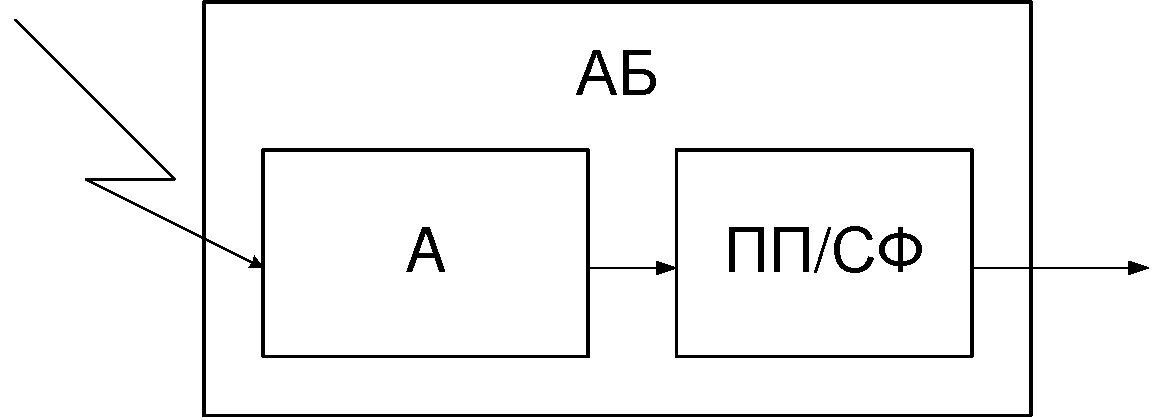
\includegraphics[scale=0.4]{ant_sns}
\caption{Схема антенного блоку СНС}
\label{fig:ant_sns}
\end{figure} 

Прийомообчислювач виконаний у вигляді блоку, у якому розташовані модулі вторинних 
джерел живлення і плати --- прийомокорелятора, навігаційного обчислювача та інтерфейсного 
пристрою (рис. \ref{fig:sns}). Вхід ПО через фідерну лінію з'єднаний з виходом антенного блоку. 
В аналоговому приймачі АП сигнали підсилюються, фільтруються і переносяться з несучої 
частоти на проміжну (зниження частоти). В аналого-цифровому перетворювачі АЦП аналоговий 
сигнал перетвориться в цифрову форму.
\begin{figure}[here]
\centering
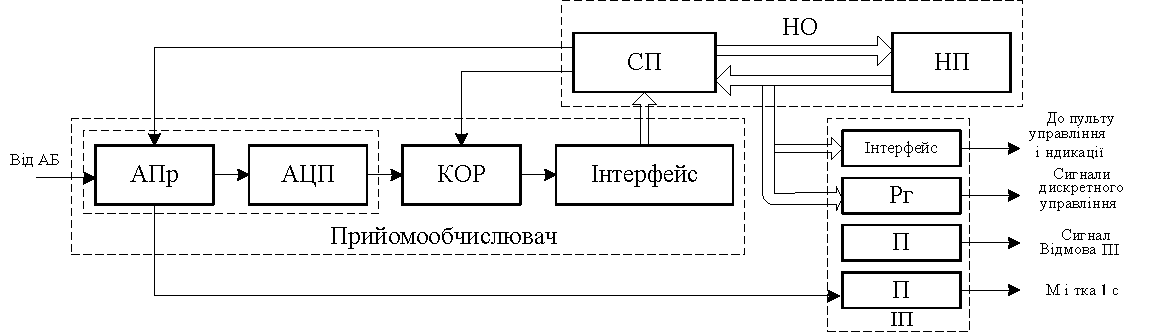
\includegraphics[scale=0.9]{sns}
\caption{Схема прийомообчислювача}
\label{fig:sns}
\end{figure} 
В кореляторі (КОР) у цифровій формі формуються синфазні  і квадратурні  відліки, що є 
основою роботи алгоритмів пошуку сигналів по затримці і частоті спостереження за псевдодальністю, 
фазою сигналу і виділення навігаційного повідомлення.

Навігаційний обчислювач НО є цифровим процесором, у якому реалізується обчислювальний процес 
і керування роботою ПІ. Навігаційний обчислювач зручно представити у виді сигнального процесора 
СП, що реалізує алгоритми первинної обробки квадратурних складових, і навігаційного процесора 
НП, що реалізує алгоритми низькочастотної обробки, тобто рішення навігаційної задачі.

У прийнятого радіосигналу виміряються затримка $\tau$ або доплерівський зсув частоти $f_{\text{доп}}$, 
які є радіонавігаційними параметрами, а відповідні їм дальність до об'єкта $D=c*\tau$  
і радіальна швидкість зближення $V_{p}=f_{\text{доп}}\lambda$   служать навігаційними параметрами 
(\textit{с } -- швидкість світла;$\lambda$ -- довжина хвилі радіосигналу).

Просторове положення споживача визначається в прийомоіндикаторі в два етапи: спочатку визначаються 
поточні координати супутників і первинні навігаційні параметри (дальність, її похідні й ін.) щодо 
відповідних НС, а потім розраховуються вторинні --- географічна широта, довгота, висота споживача і т.д.

Вектор швидкості споживача обчислюють шляхом обробки результатів вимірів доплерівських зсувів 
частоти сигналів НС з урахуванням відомого вектора швидкості супутника. 

Інтерфейсний пристрій (ІП) призначений для забезпечення взаємодії прийомоіндикатора з зовнішніми 
пристроями такими, наприклад, як пульт керування й індикації (ПКІ). Додатково до складу ІП входять 
два підсилювачі П, що формують ознаку відмови ПІ і сигнали дискретного керування, а також 8-розрядний 
регістр Рг, що приймає сигнали дискретного керування. Цей регістр доступний для читання з боку НО. 
Останній, у залежності від інформації, що знаходиться в регістрі, вибирає той або інший режим роботи.

Таким чином, основною операцією, що виконуваної в СНС за допомогою космічного сегменту, сегменту 
керування та сегменту споживача, є визначення просторових координат місця розташування споживачів і 
часу, тобто просторово-тимчасових координат (ПТК). Як було показано, цю операцію здійснюють відповідно 
до концепції незалежної навігації, що передбачає обчислення шуканих навігаційних параметрів 
безпосередньо в апаратурі споживача. У рамках цієї концепції в СРНС обраний позиційний спосіб 
визначення місця розташування споживачів на основі беззапитних (пасивних) далекомірних вимірів по 
сигналах декількох навігаційних штучних супутників Землі з відомими координатами. Висока точність 
визначення місця розташування споживачів обумовлена багатьма факторами, включаючи взаємне розташування 
супутників і параметри їхніх навігаційних сигналів. Структура космічного сегмента забезпечує для 
споживача постійну видимість необхідного числа супутників.

Використання СНС в інтересах місцезнаходження і навігації рухливих об'єктів, а також у рішенні 
спеціальних задач (спостереження, аерофотознімання, пошук корисних копалин, пошук і порятунок 
транспортних засобів, що терплять нещастя, і людей) висуває високі вимоги.

Вимоги до точнісних характеристик, таких як середньоквадратичне відхилення помилки (СКП) визначення 
навігаційних параметрів, показників надійності навігаційного забезпечення, тощо наступні:
\begin{itemize}
  \itemдоступність (готовність),  мірою якої є імовірність працездатності СРНС перед виконанням 
тієї або іншої задачі та у процесі її виконання. Чисельні значення доступності складають 0,95...\dots 0,997;
 \itemцілісність, мірою якої є імовірність виявлення відмови протягом часу, рівному заданому 
або менше. Вимоги до цілісності для маршрутних польотів складає 0,999;
 \itemбезперервність обслуговування, мірою якої служить імовірність працездатності системи 
протягом найбільш відповідальних відрізків часу. На етапах заходу на посадку вимоги до безперервності 
обслуговування складають $10^{-5}$ \dots ... $10^{-4}$ для проміжків часу від 15 до 150 с.
\end{itemize}

Основні навігаційні параметри, що визначаються в СРНС -- дальність і радіальна швидкість. Відповідними 
їм радіонавігаційними параметрами (параметрами радіосигналу) служать затримка t сигналу і доплерівський 
зсув частоти $f_\text{доп}$. Оскільки головною вимогою до СРНС є висока точність виміру 
навігаційних параметрів, отже, й основною вимогою до радіосигналів так само є висока точність 
виміру затримки t сигналу і доплерівського зсуву частоти $f_\text{доп}$.

Вимоги до підвищення точності затримки сигналу і доплерівського зсуву частоти суперечливі. 
Для підвищення точності виміру затримки необхідно розширювати спектр сигналу, а для підвищення 
точності виміру  доплерівського зсуву частоти --  збільшувати тривалість сигналу.

Дане протиріччя вирішується при вирішенні задачі спільної оцінки t та  $f_\text{доп}$.

Підвищення точності спільних оцінок затримки сигналу і доплерівського зсуву частоти можна 
досягти за рахунок збільшення так званої  бази сигналу -- \textit{В}(добуток ефективної 
тривалості сигналу на ефективну ширину спектра сигналу) і основною вимогою до радіосигналів у 
СРНС є збільшення бази сигналу $В>>1$. Такі сигнали називають шумоподібними. 
Відомо, що стійкість до перешкод радіотехнічної системи визначається значенням бази сигналу, 
а для більшості ЛА скритність і перешкодозахищеність є одним з визначальних вимог. 

Інша істотна вимога --- забезпечення багатостанційного доступу. При визначенні навігаційних 
параметрів у споживача повинна бути можливість одночасного доступу до сигналів від різних 
супутників. Проблема багатостанційного доступу вирішується шляхом тимчасового, частотного 
або кодового поділу сигналів, наприклад, у супутниковій навігаційній системі GPS використовується 
кодовий поділ, у СРНС ГЛОНАСС - частотний.

З результатів аналізів стає очевидно, що не має принципової різниці між супутниковими 
навігаційними системами GPS та ГЛОНАСС.

В залежності від області використання апаратура споживача (АС) має свої особливості, 
тому виробники АС завжди вказують на область застосування відповідного зразка. Крім 
основних блоків, таких, як антена, приймач, індикатор, АС може містити допоміжні, що 
забезпечують виконання спеціальних сервісних функцій, наприклад, діагностику вузлів 
транспортного засобу, зв'язок з диспетчерським пунктом і т.п.

В табл. \ref{tb:ac} наведені коротка інформація про основні зразки АС, що працюють за сигналами 
СРНС ГЛОНАСС та GPS. Наведена інформація не претендує на повноту відомостей як про існуючі 
зразки АС, так і про іх характеристики, а дається для ілюстрації досягнутого рівня 
в розробці та виробництві АС СРНС.
Апаратура споживачів
\begin{table}[here]
\small
\caption{Апаратура споживачів}
\centering
\begin{tabular}{|p{30mm}|p{20mm}|p{20mm}|p{20mm}|p{20mm}|p{20mm}|p{10mm}|} \hline 
Найменування апаратури & Область використання & Виробник & Число каналів & 
\multicolumn{2}{|p{30mm}|}{Точність (в автономному режимі)} & Маса, кг \\ \hline 
 &  &  &  & координат, м & швидкості, м/с &  \\ \hline 
Станція моніторингу та формування ДП & Моніторинг & РНИИ КЛ & 24 & 1...3 & 1...2 & 6,0 \\ \hline 
„Гном-М'' & Авіація &  & 6...12 & 80...90 & 12...15 & 3,2 \\ \hline 
АСН-22 & Авіація & РИРВ & 18 & 25...30 &  & 0,4 \\ \hline 
НАВИС СН 3301 & Авіація &  & 14 & 15...20 & 8...10 & 2,4 \\ \hline 
„Интер-А'' & Авіація & МКБ КОМПАС & 12 & 25...30 & 10...30 & 3,5 \\ \hline 
А-744 & Авіація & Фирма „Кодтик'' & 6 & 30...35 & 15...20 & 2,0 \\ \hline 
\end{tabular}
\label{tb:ac}
\end{table}

З огляду на, те що  супутникова система навігації буде працювати в комплексі з 
інерціальною системою навігації, то навряд варто встановлювати  на борт ЛА повний 
комплект супутникової системи. Досить обмежитися  прийомоіндикатором і сигнальним 
процесором, думаючи, що алгоритми рішення навігаційної задачі будуть вирішуватися 
в спільному процесорі інерціально - супутникової системи навігації. 

Виходячи з вищенаведеного, а також враховуючи умови застосування ЛА та вимоги 
ТЗ можна сформулювати вимоги, яким повинний задовольняти обраний тип прийомоіндикатора 
СРНС. 

Розв'язувані задачі:
\begin{itemize}
\item автоматичне, безперервне, глобальне, всепогодне визначення поточних ЗD-координат 
місця розташування, вектора шляхової швидкості шляхового кута ЛА при роботі: по 
сигналу стандартної точності частотного діапазону L1 ГЛОНАСС; по сигналі З/А-коду 
GPS; при спільній обробці вищевказаних сигналів;
\item видача поточних ЗD-координат місця розташування ЛА, що є складовими вектора 
швидкості і шляхового кута в системі координат СК-42 або ПЗ-90 у географічному 
форматі, а також ознак режиму роботи апаратури;
\item стійке визначення навігаційних параметрів при русі з лінійними прискореннями 
і при стрибкоподібних змінах прискорення;
\item  можливість переключення з антени носія на антену ЛА; 
\item інтегральна оцінка очікуваної точності визначення поточних координат місця розташування;
\item автоматичний вибір оптимального з погляду очікуваної точності сузір'я НС ГЛОНАСС і GPS при роботі в сполученому режимі;
\item автоматичне рішення навігаційної задачі в географічній системі координат:  
\end{itemize}